% =============================================================================
% sections/design/rover/critical_parts/rocker_suspension.tex  -  Rocker-Only Suspension
% Teams: suspension (best guess - unconfirmed) / Status: stub
%
% Content required:
%   - How this suspension suits us; its obstacle-overcoming capabilities
%   - Scheme with sizes
%   - Photo of suspension
%   - Photo of overcoming obstacles
% Evidence-first rule (ai_context/DECISIONS.md): lead with the
% scheme/photos, keep prose to what the figures cannot say.
% =============================================================================

\todo[inline]{How this rocker-only suspension suits us, and its
obstacle-overcoming capabilities. Maximum obstacle height, turning radiuses, maximum slope will be specified here.}

\begin{figure}[!htbp]
    \centering
    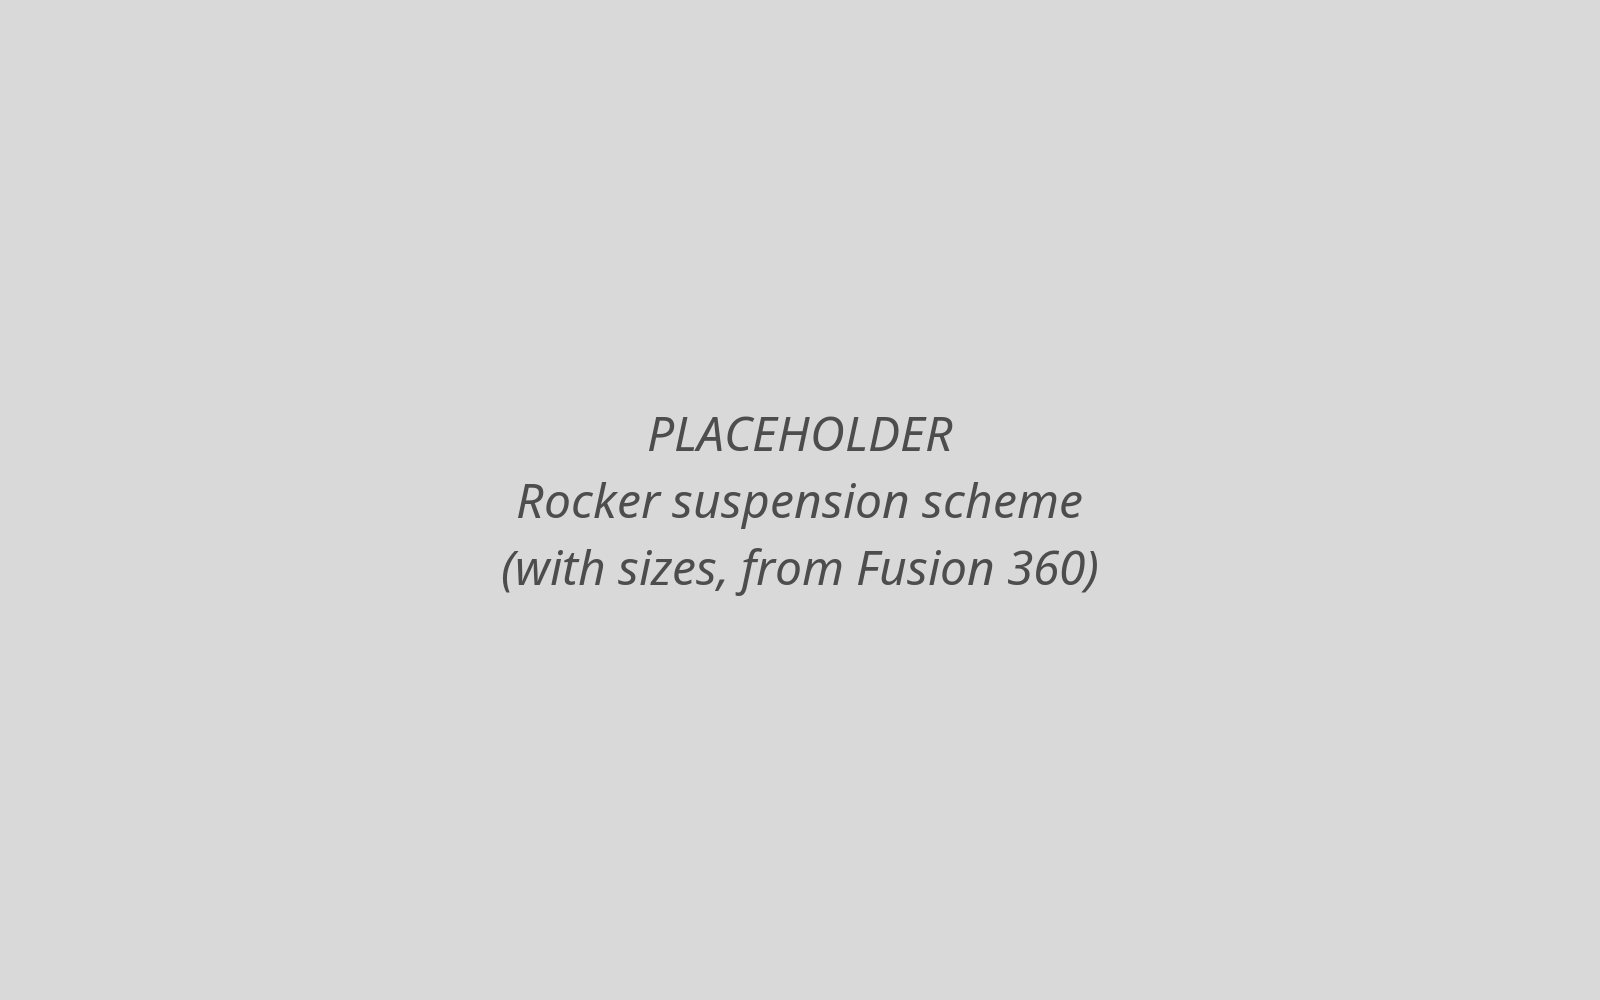
\includegraphics[width=0.8\linewidth]{teams/suspension/figures/rocker_suspension_scheme}
    \caption{Rocker suspension scheme with sizes (Fusion 360)}\label{fig:rocker_suspension_scheme}
\end{figure}

\begin{figure}[!htbp]
    \centering
    \begin{subfigure}[b]{0.48\textwidth}
        \centering
        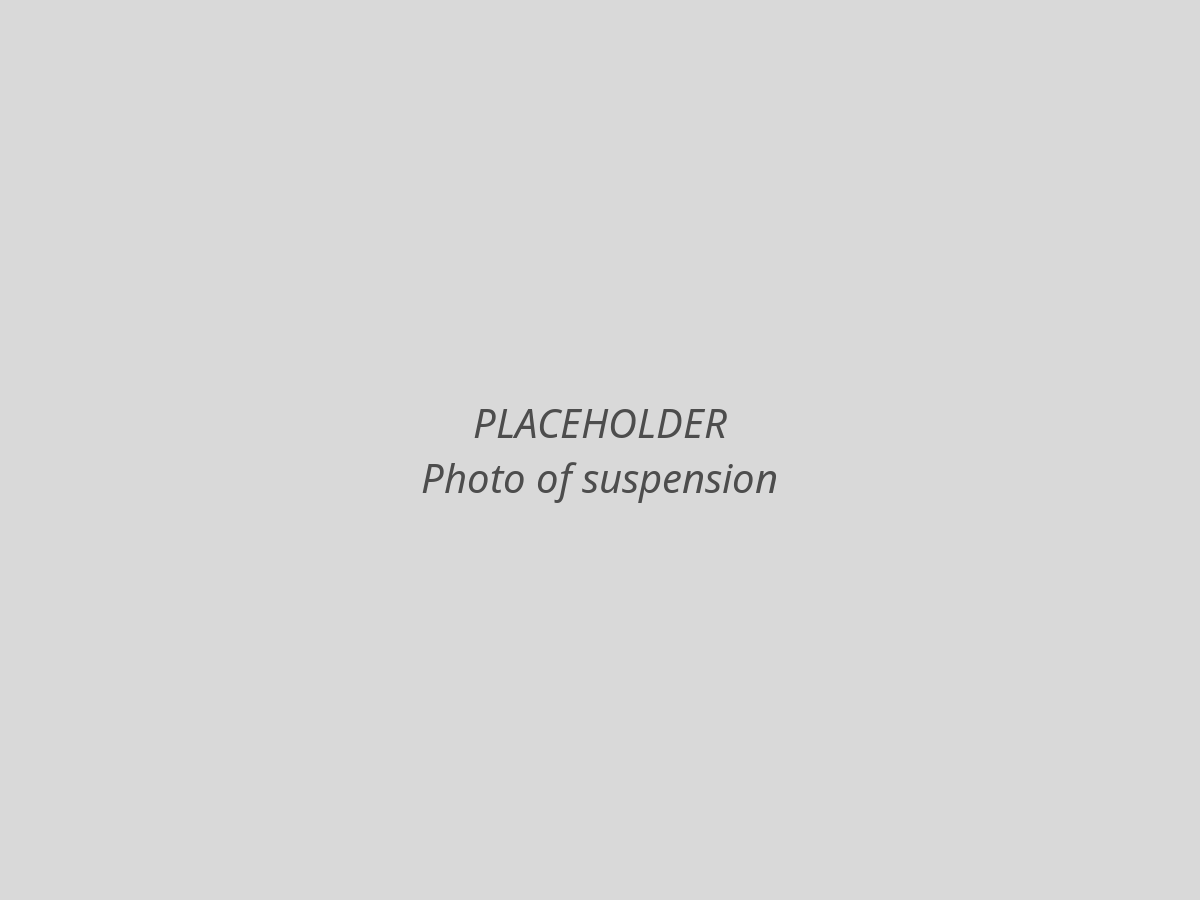
\includegraphics[width=\linewidth]{teams/suspension/figures/rocker_suspension_photo}
        \caption{Photo of suspension}
    \end{subfigure}
    \hfill
    \begin{subfigure}[b]{0.48\textwidth}
        \centering
        
\includegraphics[width=\linewidth]{teams/suspension/figures/rocker_suspension_obstacle}
        \caption{Photo of overcoming obstacles}
    \end{subfigure}
    \caption{Rocker suspension in operation}\label{fig:rocker_suspension_operation}
\end{figure}
